% Similarity of Triangles — Quick Notes (Grade 10)
\documentclass[11pt,a4paper]{article}

% Packages per requirements
\usepackage[margin=1in]{geometry}
\usepackage[T1]{fontenc}
\usepackage[utf8]{inputenc}
\usepackage{microtype}
\usepackage[dvipsnames]{xcolor}
\usepackage{hyperref}
\usepackage{amsmath,amssymb,mathtools}
\usepackage{tcolorbox}
% Load tcolorbox libraries for enhanced and breakable boxes
\tcbuselibrary{skins,breakable}
\usepackage{tikz}
\usepackage{enumitem}
\usepackage{multicol}
\usepackage{tabularx}
\usepackage{booktabs}
\usepackage{graphicx}
\usepackage{newtxtext,newtxmath}

% TikZ libraries and styles
\usetikzlibrary{angles,quotes,calc,arrows.meta}
\tikzset{
  side/.style={draw=RoyalBlue, line width=1.1pt},
  parallel/.style={draw=Fuchsia, line width=1.1pt, dash pattern=on 4pt off 3pt},
  angmark/.style={draw=ForestGreen, line width=1pt},
  rightmark/.style={draw=ForestGreen, line width=1pt},
  label/.style={black, font=\footnotesize},
  tick/.style={draw=Gray, line width=0.6pt},
  arrow/.style={-Stealth, draw=BrickRed, line width=0.9pt}
}

% Hyperref setup
\hypersetup{
  colorlinks=true,
  linkcolor=BrickRed,
  urlcolor=RoyalBlue,
  citecolor=ForestGreen,
  pdfauthor={Quick Notes},
  pdftitle={Similarity of Triangles — Quick Notes (Grade 10)}
}

% Header and footer
\pagestyle{myheadings}
\markright{Similarity of Triangles — Quick Notes (Grade 10)}

% Lists spacing
\setlist{itemsep=0.25em, topsep=0.3em, parsep=0em, partopsep=0em, leftmargin=1.2em}

% tcolorbox styles
\tcbset{sharp corners, boxrule=0.9pt, enhanced, breakable}

\newtcolorbox{definitionbox}[1][]{colback=RoyalBlue!4, colframe=RoyalBlue!70!black, coltitle=black, title=Definition, #1}
\newtcolorbox{theorembox}[1][]{colback=ForestGreen!4, colframe=ForestGreen!70!black, coltitle=black, title=Theorem/Rule, #1}
\newtcolorbox{propertybox}[1][]{colback=Gray!8, colframe=Gray!70!black, coltitle=black, title=Property, #1}
\newtcolorbox{examplebox}[1][]{colback=RoyalBlue!2, colframe=RoyalBlue!60!black, coltitle=black, title=Example, #1}
\newtcolorbox{shortcutbox}[1][]{colback=Goldenrod!8, colframe=Goldenrod!60!black, coltitle=black, title=Shortcut, #1}
\newtcolorbox{warningbox}[1][]{colback=BrickRed!6, colframe=BrickRed!80!black, coltitle=black, title=Warning, #1}

% Small helpers
\newcommand{\vect}[1]{\overrightarrow{#1}}
\newcommand{\ratio}{\ensuremath{\,\raisebox{0.3ex}{:}\,}}

\begin{document}

%========================
% Title Page
%========================
\begin{titlepage}
  \centering
  \vspace*{2.5cm}
  {\Huge \bfseries Similarity of Triangles\\[6pt] \Large Quick Notes (Grade 10)}\\[1.2cm]
  {\large Clean, colorful, exam-ready}\par
  \vfill

  % Color legend
  \begin{minipage}{0.9\textwidth}
    \begin{multicols}{2}
      \begin{definitionbox}
        Use for: precise meanings and notation.
      \end{definitionbox}
      \begin{theorembox}
        Use for: key rules and criteria.
      \end{theorembox}
      \begin{propertybox}
        Use for: consequences and facts.
      \end{propertybox}
      \begin{examplebox}
        Use for: worked examples with steps.
      \end{examplebox}
      \begin{shortcutbox}
        Use for: quick tricks and checks.
      \end{shortcutbox}
      \begin{warningbox}
        Use for: common mistakes and alerts.
      \end{warningbox}
    \end{multicols}
  \end{minipage}

  \vfill
  {\small Sides in RoyalBlue, angle marks in ForestGreen, parallels in Fuchsia.}\par
  \vspace*{1cm}
  {\small \textcopyright\ \the\year}\par
  \thispagestyle{empty}
\end{titlepage}

\setcounter{page}{1}

%========================
% One-Page Overview
%========================
\section*{Overview: What is Similarity?}
\begin{multicols}{2}
\begin{definitionbox}
Two figures are \textbf{similar} if they have the same shape. For triangles, this means:
\begin{itemize}
  \item Corresponding \textbf{angles are equal}.
  \item Corresponding \textbf{side lengths are in proportion}.
\end{itemize}
We write: $\triangle ABC \sim \triangle A'B'C'$.
\end{definitionbox}

\begin{propertybox}
\textbf{Scale factor $k$:} If $\triangle ABC \sim \triangle A'B'C'$, and $AB$ matches $A'B'$, then $\dfrac{A'B'}{AB} = k$. Every corresponding side scales by $k$.
\begin{itemize}
  \item Perimeters scale by $k$.
  \item Areas scale by $k^2$.
\end{itemize}
\end{propertybox}

\begin{examplebox}
\textbf{Matching corresponding parts:} Keep vertex order consistent. If $\triangle ABC \sim \triangle DEF$, then $A\leftrightarrow D$, $B\leftrightarrow E$, $C\leftrightarrow F$. So $\dfrac{AB}{DE}=\dfrac{BC}{EF}=\dfrac{CA}{FD}$.
\end{examplebox}

\begin{shortcutbox}
\textbf{Quick check:} If two angles of one triangle match two of another, triangles are similar (AAA). You do not need the third angle.
\end{shortcutbox}

\begin{center}
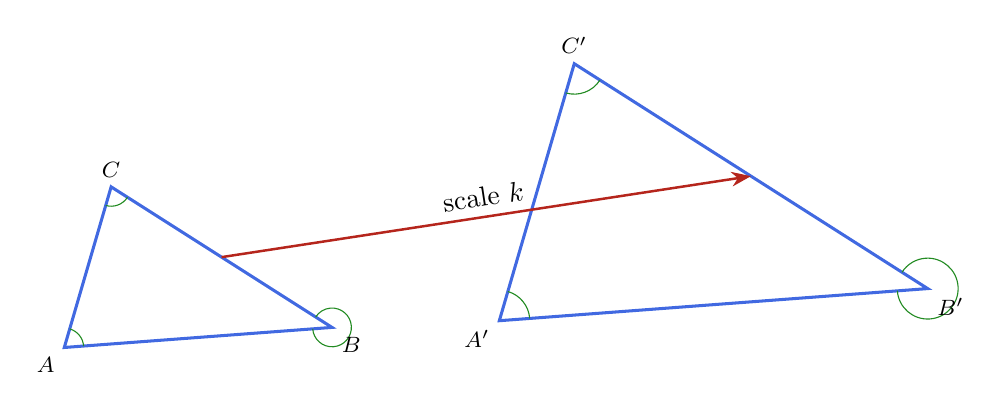
\begin{tikzpicture}[scale=0.85]
  % Triangle ABC
  \coordinate (A) at (0,0);
  \coordinate (B) at (4,0.3);
  \coordinate (C) at (0.7,2.4);
  \draw[side] (A)--(B)--(C)--cycle;
  % Angle marks ABC
  \pic[draw=ForestGreen, angle radius=7pt, angle eccentricity=1.1]{angle=B--A--C};
  \pic[draw=ForestGreen, angle radius=7pt]{angle=A--B--C};
  \pic[draw=ForestGreen, angle radius=7pt]{angle=A--C--B};
  \node[label] at (A) [below left] {$A$};
  \node[label] at (B) [below right] {$B$};
  \node[label] at (C) [above] {$C$};

  % Triangle A'B'C' scaled by k=1.6
  \coordinate (Ap) at (6.5,0.4);
  \coordinate (Bp) at ($(Ap)+(1.6*4,1.6*0.3)$);
  \coordinate (Cp) at ($(Ap)+(1.6*0.7,1.6*2.4)$);
  \draw[side] (Ap)--(Bp)--(Cp)--cycle;
  \pic[draw=ForestGreen, angle radius=11pt]{angle=Bp--Ap--Cp};
  \pic[draw=ForestGreen, angle radius=11pt]{angle=A--Bp--Cp};
  \pic[draw=ForestGreen, angle radius=11pt]{angle=Ap--Cp--Bp};
  \node[label] at (Ap) [below left] {$A'$};
  \node[label] at (Bp) [below right] {$B'$};
  \node[label] at (Cp) [above] {$C'$};

  \draw[arrow] ($(B)!0.5!(C)$) -- node[above, sloped]{scale $k$} ($(Bp)!0.5!(Cp)$);
\end{tikzpicture}
\end{center}

\begin{warningbox}
\textbf{Keep order:} $\triangle ABC\sim\triangle DEF$ means $A\leftrightarrow D$, $B\leftrightarrow E$, $C\leftrightarrow F$. Mixing order gives wrong ratios.
\end{warningbox}
\end{multicols}

\newpage

%========================
% Core Definitions and Criteria
%========================
\section*{Core Definitions and Similarity Criteria}

\begin{definitionbox}
\textbf{Similar triangles:} $\triangle ABC \sim \triangle A'B'C'$ if $\angle A = \angle A'$, $\angle B = \angle B'$, $\angle C = \angle C'$ (AAA), or if certain side-angle conditions hold (SAS, SSS).
\end{definitionbox}

\begin{multicols}{3}
\begin{theorembox}
\textbf{AAA Similarity}
\begin{itemize}
  \item If three angles of a triangle match the three angles of another, the triangles are similar.
  \item Ratios of corresponding sides are equal.
\end{itemize}
\begin{center}
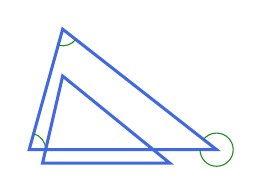
\begin{tikzpicture}[scale=0.85]
  \coordinate (A) at (0,0);
  \coordinate (B) at (2.8,0);
  \coordinate (C) at (0.5,1.8);
  \draw[side] (A)--(B)--(C)--cycle;
  \pic[draw=ForestGreen, angle radius=6pt]{angle=B--A--C};
  \pic[draw=ForestGreen, angle radius=6pt]{angle=A--B--C};
  \pic[draw=ForestGreen, angle radius=6pt]{angle=A--C--B};
  \coordinate (Ap) at (0.2,-0.2);
  \coordinate (Bp) at (2.1,-0.2);
  \coordinate (Cp) at (0.5,1.1);
  \draw[side] (Ap)--(Bp)--(Cp)--cycle;
\end{tikzpicture}
\end{center}
\end{theorembox}

\columnbreak

\begin{theorembox}
\textbf{SAS Similarity}
\begin{itemize}
  \item Two sides in proportion and the included angle equal imply similarity.
  \item $\dfrac{AB}{A'B'} = \dfrac{AC}{A'C'}$ and $\angle A = \angle A'$.
\end{itemize}
\begin{center}
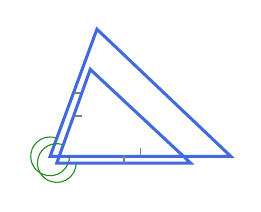
\begin{tikzpicture}[scale=0.85]
  \coordinate (A) at (0,0);
  \coordinate (B) at (2.7,0);
  \coordinate (C) at (0.7,1.9);
  \draw[side] (A)--(B)--(C)--cycle;
  \draw[tick] ($(A)!0.5!(B)$) -- ++(0,0.12);
  \draw[tick] ($(A)!0.5!(C)$) -- ++(0.12,0);
  \pic[draw=ForestGreen, angle radius=7pt]{angle=C--A--B};
  \coordinate (Ap) at (0.1,-0.1);
  \coordinate (Bp) at (2.1,-0.1);
  \coordinate (Cp) at (0.6,1.3);
  \draw[side] (Ap)--(Bp)--(Cp)--cycle;
  \draw[tick] ($(Ap)!0.5!(Bp)$) -- ++(0,0.12);
  \draw[tick] ($(Ap)!0.5!(Cp)$) -- ++(0.12,0);
  \pic[draw=ForestGreen, angle radius=7pt]{angle=C--Ap--Bp};
\end{tikzpicture}
\end{center}
\end{theorembox}

\columnbreak

\begin{theorembox}
\textbf{SSS Similarity}
\begin{itemize}
  \item All three side pairs are in the same ratio $k$.
  \item $\dfrac{AB}{A'B'} = \dfrac{BC}{B'C'} = \dfrac{CA}{C'A'} = k$.
\end{itemize}
\begin{center}
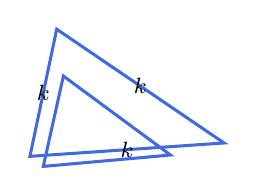
\begin{tikzpicture}[scale=0.85]
  \coordinate (A) at (0,0);
  \coordinate (B) at (2.9,0.2);
  \coordinate (C) at (0.4,1.9);
  \draw[side] (A)--(B)--(C)--cycle;
  \node[label] at ($(A)!0.5!(B)$) {$k$};
  \node[label] at ($(B)!0.5!(C)$) {$k$};
  \node[label] at ($(C)!0.5!(A)$) {$k$};
  \coordinate (Ap) at (0.2,-0.15);
  \coordinate (Bp) at (2.1,0.02);
  \coordinate (Cp) at (0.5,1.2);
  \draw[side] (Ap)--(Bp)--(Cp)--cycle;
\end{tikzpicture}
\end{center}
\end{theorembox}
\end{multicols}

\begin{warningbox}
\textbf{Common mistakes}
\begin{itemize}
  \item Using a non-included angle for SAS.
  \item Mismatching corresponding sides when writing ratios.
  \item Forgetting that areas scale by $k^2$, not by $k$.
\end{itemize}
\end{warningbox}

\newpage

%========================
% Consequences of Similarity
%========================
\section*{Consequences of Similarity}

\begin{propertybox}
If $\triangle ABC \sim \triangle A'B'C'$ with scale factor $k$ (so $A'B' = k\,AB$), then:
\begin{itemize}
  \item Corresponding angles are equal.
  \item $\dfrac{AB}{A'B'} = \dfrac{BC}{B'C'} = \dfrac{CA}{C'A'} = \dfrac{1}{k}$.
  \item Perimeter ratio is $\dfrac{P_{A'B'C'}}{P_{ABC}} = k$.
  \item Area ratio is $\dfrac{[A'B'C']}{[ABC]} = k^2$.
  \item Altitudes, medians, and angle bisectors scale by $k$.
\end{itemize}
\end{propertybox}

\begin{examplebox}
\textbf{A quick proof (altitudes scale by $k$)}: In similar triangles, $\dfrac{AB}{A'B'} = \dfrac{h_{AB}}{h'_{A'B'}}$ because both pairs are opposite equal angles and form similar right triangles when dropping perpendiculars. Hence $h'_{A'B'} = k\,h_{AB}$.
\end{examplebox}

\begin{center}
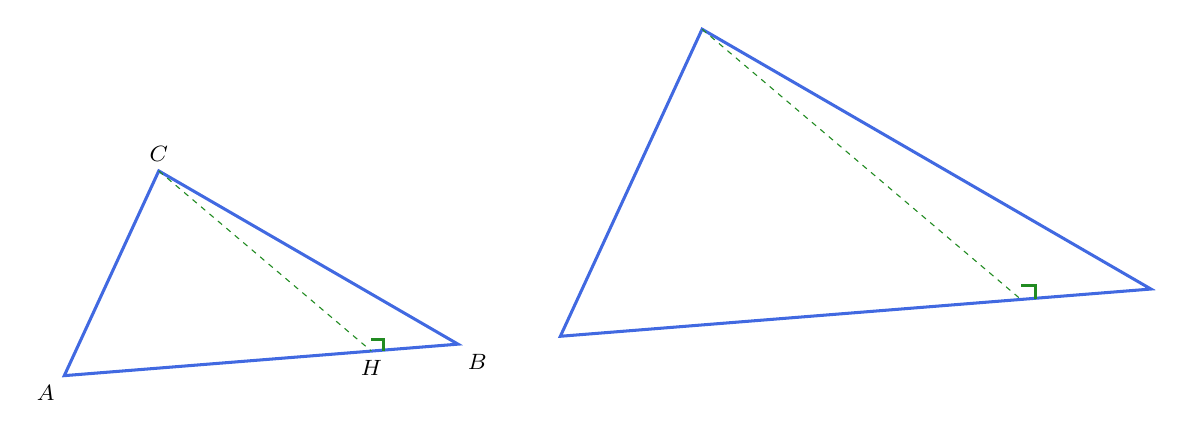
\begin{tikzpicture}[scale=1]
  % Triangle ABC with altitude
  \coordinate (A) at (0,0);
  \coordinate (B) at (5,0.4);
  \coordinate (C) at (1.2,2.6);
  \draw[side] (A)--(B)--(C)--cycle;
  % altitude from C to AB
  \coordinate (H) at ($(A)!0.78!(B)$);
  \draw[ForestGreen, dash pattern=on 2pt off 2pt] (C) -- (H);
  \draw[rightmark] ($(H)+(0.15,0)$) -- ++(0,0.15) -- ++(-0.15,0);
  \node[label] at (H) [below] {$H$};
  \node[label] at (A) [below left] {$A$};
  \node[label] at (B) [below right] {$B$};
  \node[label] at (C) [above] {$C$};

  % Scaled triangle A'B'C'
  \coordinate (Ap) at (6.3,0.5);
  \coordinate (Bp) at ($(Ap)+(1.5*5,1.5*0.4)$);
  \coordinate (Cp) at ($(Ap)+(1.5*1.2,1.5*2.6)$);
  \draw[side] (Ap)--(Bp)--(Cp)--cycle;
  \coordinate (Hp) at ($(Ap)!0.78!(Bp)$);
  \draw[ForestGreen, dash pattern=on 2pt off 2pt] (Cp) -- (Hp);
  \draw[rightmark] ($(Hp)+(0.18,0)$) -- ++(0,0.18) -- ++(-0.18,0);
\end{tikzpicture}
\end{center}

\begin{shortcutbox}
\textbf{Area shortcut:} If sides scale by $k$, areas scale by $k^2$. If perimeters scale by $3$, areas scale by $9$.
\end{shortcutbox}

\newpage

%========================
% Key Theorems via Similarity
%========================
\section*{Key Theorems from Similarity}

\begin{theorembox}
\textbf{Basic Proportionality Theorem (Thales)}: If a line through a triangle is parallel to one side, it divides the other two sides proportionally.

If $DE \parallel BC$ in $\triangle ABC$, then $\dfrac{AD}{DB} = \dfrac{AE}{EC}$ and $\dfrac{AD}{AB} = \dfrac{AE}{AC}$.
\end{theorembox}

\begin{center}
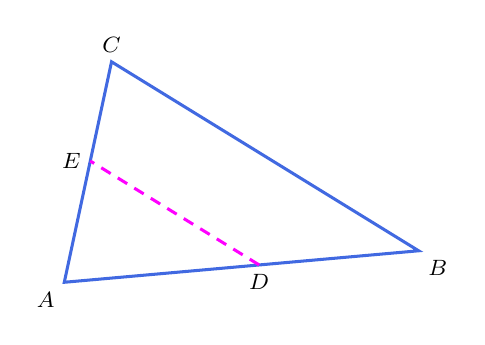
\begin{tikzpicture}[scale=1]
  \coordinate (A) at (0,0);
  \coordinate (B) at (4.5,0.4);
  \coordinate (C) at (0.6,2.8);
  \draw[side] (A)--(B)--(C)--cycle;
  \coordinate (D) at ($(A)!0.55!(B)$);
  \coordinate (E) at ($(A)!0.55!(C)$);
  \draw[parallel] (D)--(E);
  \node[label] at (A) [below left] {$A$};
  \node[label] at (B) [below right] {$B$};
  \node[label] at (C) [above] {$C$};
  \node[label] at (D) [below] {$D$};
  \node[label] at (E) [left] {$E$};
\end{tikzpicture}
\end{center}

\begin{examplebox}
\textbf{Proof idea:} Since $DE\parallel BC$, $\angle ADE = \angle ABC$ and $\angle AED = \angle ACB$ (alternate interior angles). Thus $\triangle ADE \sim \triangle ABC$ (AAA), so $\dfrac{AD}{AB} = \dfrac{AE}{AC}$ and $\dfrac{DE}{BC} = \dfrac{AD}{AB} = \dfrac{AE}{AC}$. From the first, \(\dfrac{AD}{DB} = \dfrac{AE}{EC}\).
\end{examplebox}

\begin{theorembox}
\textbf{Converse of BPT}: If a line through a triangle cuts two sides proportionally, it is parallel to the third side.
\end{theorembox}

\begin{theorembox}
\textbf{Angle Bisector Theorem (internal)}: In $\triangle ABC$, if $AD$ bisects $\angle A$ with $D$ on $BC$, then $\dfrac{BD}{DC} = \dfrac{AB}{AC}$.

\textbf{External} bisector at $A$ meets the extension of $BC$ at $E$ and gives $\dfrac{BE}{EC} = \dfrac{AB}{AC}$.
\end{theorembox}

\begin{center}
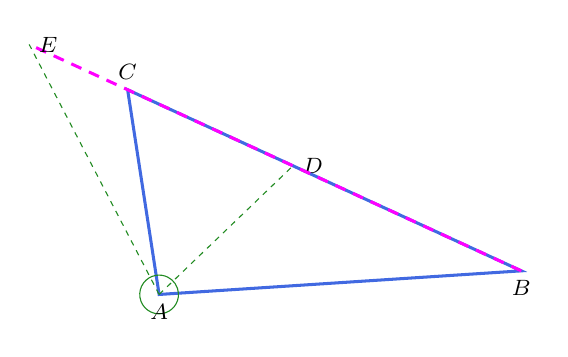
\begin{tikzpicture}[scale=1]
  \coordinate (A) at (0.4,0);
  \coordinate (B) at (5,0.3);
  \coordinate (C) at (0,2.6);
  \draw[side] (A)--(B)--(C)--cycle;
  % Internal bisector AD
  \coordinate (D) at ($(B)!0.58!(C)$);
  \draw[ForestGreen, dash pattern=on 2pt off 2pt] (A)--(D);
  \pic[draw=ForestGreen, angle radius=7pt]{angle=C--A--B};
  \pic[draw=ForestGreen, angle radius=7pt]{angle=B--A--C};
  \node[label] at (A) [below] {$A$};
  \node[label] at (B) [below] {$B$};
  \node[label] at (C) [above] {$C$};
  \node[label] at (D) [right] {$D$};

  % External bisector AE
  \coordinate (E) at ($(B)!1.25!(C)$);
  \draw[ForestGreen, dash pattern=on 2pt off 2pt] (A)--(E);
  \draw[parallel] (B)--(E);
  \node[label] at (E) [right] {$E$};
\end{tikzpicture}
\end{center}

\begin{examplebox}
\textbf{Right-triangle similarity facts:}
\begin{itemize}
  \item In right $\triangle ABC$ with right angle at $C$, altitude from $C$ to hypotenuse $AB$ meets $AB$ at $H$. Then $\triangle ACH \sim \triangle ABC \sim \triangle HCB$.
  \item Mean proportionals: $CH^2 = AH\cdot HB$, $AC^2 = AH\cdot AB$, $BC^2 = HB\cdot AB$.
  \item \textbf{Pythagoras by similarity:} From $AC^2 = AH\cdot AB$ and $BC^2 = HB\cdot AB$, add to get $AC^2 + BC^2 = (AH+HB)\cdot AB = AB^2$.
\end{itemize}
\end{examplebox}

\begin{center}
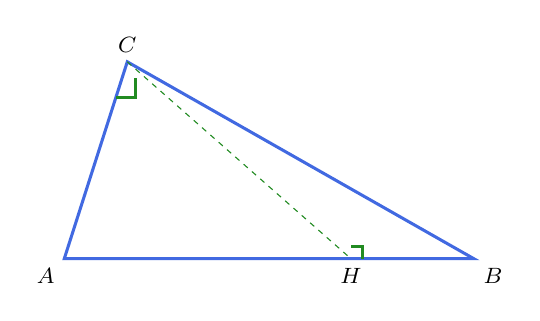
\begin{tikzpicture}[scale=1]
  \coordinate (A) at (0,0);
  \coordinate (B) at (5.2,0);
  \coordinate (C) at (0.8,2.5);
  \draw[side] (A)--(B)--(C)--cycle;
  % Right angle at C
  \draw[rightmark] ($(C)!0.18!(A)$) -- ++(0.25,0) -- ++(0,0.25);
  % Altitude to hypotenuse
  \coordinate (H) at ($(A)!0.7!(B)$);
  \draw[ForestGreen, dash pattern=on 2pt off 2pt] (C)--(H);
  \draw[rightmark] ($(H)+(0.15,0)$) -- ++(0,0.15) -- ++(-0.15,0);
  \node[label] at (A) [below left] {$A$};
  \node[label] at (B) [below right] {$B$};
  \node[label] at (C) [above] {$C$};
  \node[label] at (H) [below] {$H$};
\end{tikzpicture}
\end{center}

\newpage

%========================
% Worked Examples
%========================
\section*{Worked Examples}

% Type A
\begin{examplebox}
\textbf{Type A: Find an unknown side using similarity}

In $\triangle ABC$, $DE\parallel BC$ with $D$ on $AB$ and $E$ on $AC$. If $AD=6$, $AB=9$, and $AE=8$, find $AC$.

\begin{center}
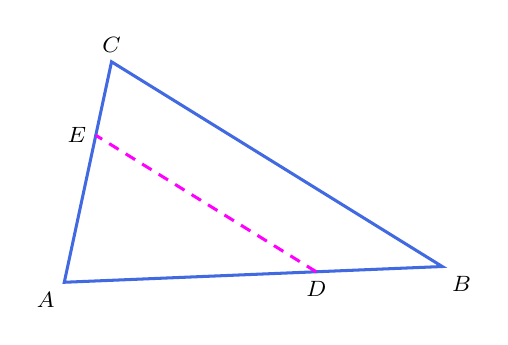
\begin{tikzpicture}[scale=1]
  \coordinate (A) at (0,0);
  \coordinate (B) at (4.8,0.2);
  \coordinate (C) at (0.6,2.8);
  \draw[side] (A)--(B)--(C)--cycle;
  \coordinate (D) at ($(A)!{6/9}!(B)$);
  \coordinate (E) at ($(A)!{8/12}!(C)$); % placeholder AC 12 to show proportional line
  \draw[parallel] (D)--(E);
  \node[label] at (A) [below left] {$A$};
  \node[label] at (B) [below right] {$B$};
  \node[label] at (C) [above] {$C$};
  \node[label] at (D) [below] {$D$};
  \node[label] at (E) [left] {$E$};
\end{tikzpicture}
\end{center}

\textbf{Steps}
\begin{enumerate}
  \item $DE\parallel BC \Rightarrow \triangle ADE \sim \triangle ABC$.
  \item $\dfrac{AD}{AB} = \dfrac{AE}{AC} \Rightarrow \dfrac{6}{9} = \dfrac{8}{AC}$.
  \item Cross-multiply: $6\,AC = 9\cdot 8 = 72$.
  \item $AC = 12$.
\end{enumerate}

\begin{shortcutbox}
Use BPT: a single proportion solves it.
\end{shortcutbox}
\end{examplebox}

% Type B
\begin{examplebox}
\textbf{Type B: Perimeter and area comparisons}

Two similar triangles have side ratio $k=\dfrac{5}{3}$. If the smaller has perimeter $24$ and area $54$, find the larger's perimeter and area.

\textbf{Steps}
\begin{enumerate}
  \item Perimeter scales by $k$: $P_{\text{large}} = k\cdot 24 = \dfrac{5}{3}\cdot 24 = 40$.
  \item Area scales by $k^2$: $A_{\text{large}} = k^2\cdot 54 = \left(\dfrac{5}{3}\right)^2 54 = \dfrac{25}{9}\cdot 54 = 150$.
\end{enumerate}

\begin{shortcutbox}
Perimeter $\times k$, area $\times k^2$. Keep which triangle is larger consistent.
\end{shortcutbox}
\end{examplebox}

% Type C
\begin{examplebox}
\textbf{Type C: Angle-bisector splits a side}

In $\triangle ABC$, $AD$ bisects $\angle A$. If $AB=7$, $AC=9$, and $BC=12$, find $BD$ and $DC$.

\begin{center}
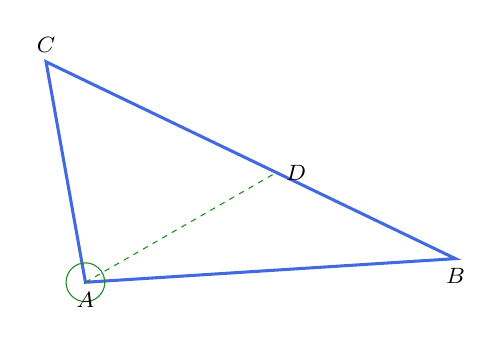
\begin{tikzpicture}[scale=1]
  \coordinate (A) at (0.5,0);
  \coordinate (B) at (5.2,0.3);
  \coordinate (C) at (0,2.8);
  \draw[side] (A)--(B)--(C)--cycle;
  \coordinate (D) at ($(B)!{7/(7+9)}!(C)$);
  \draw[ForestGreen, dash pattern=on 2pt off 2pt] (A)--(D);
  \pic[draw=ForestGreen, angle radius=7pt]{angle=C--A--B};
  \pic[draw=ForestGreen, angle radius=7pt]{angle=B--A--C};
  \node[label] at (A) [below] {$A$};
  \node[label] at (B) [below] {$B$};
  \node[label] at (C) [above] {$C$};
  \node[label] at (D) [right] {$D$};
\end{tikzpicture}
\end{center}

\textbf{Steps}
\begin{enumerate}
  \item Angle Bisector Theorem: $\dfrac{BD}{DC} = \dfrac{AB}{AC} = \dfrac{7}{9}$.
  \item Let $BD=7x$, $DC=9x$, then $7x+9x=12\Rightarrow x=\dfrac{12}{16}=\dfrac{3}{4}$.
  \item $BD=7x=5.25$, $DC=9x=6.75$.
\end{enumerate}

\begin{shortcutbox}
Split in the ratio of the adjacent sides.
\end{shortcutbox}
\end{examplebox}

% Type D
\begin{examplebox}
\textbf{Type D: Parallel line cuts triangle}

In $\triangle ABC$, $DE\parallel BC$ with $AD=5$, $DB=7$, $AE=6$. Find $EC$.

\begin{center}
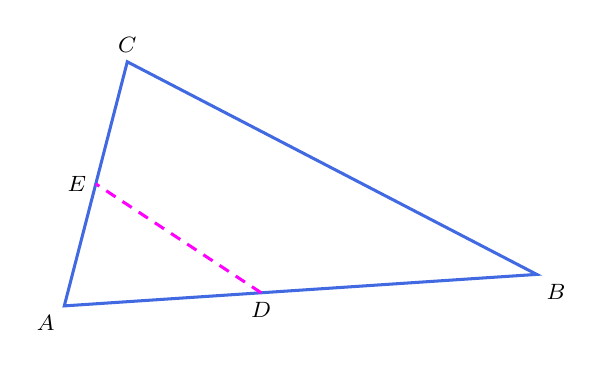
\begin{tikzpicture}[scale=1]
  \coordinate (A) at (0,0);
  \coordinate (B) at (6,0.4);
  \coordinate (C) at (0.8,3.1);
  \draw[side] (A)--(B)--(C)--cycle;
  \coordinate (D) at ($(A)!{5/(5+7)}!(B)$);
  \path let \p1=(C), \p2=(A) in coordinate (E) at ($(A)!{6/12}!(C)$); % placeholder to place E visually
  \draw[parallel] (D)--(E);
  \node[label] at (A) [below left] {$A$};
  \node[label] at (B) [below right] {$B$};
  \node[label] at (C) [above] {$C$};
  \node[label] at (D) [below] {$D$};
  \node[label] at (E) [left] {$E$};
\end{tikzpicture}
\end{center}

\textbf{Steps}
\begin{enumerate}
  \item BPT: $\dfrac{AD}{DB} = \dfrac{AE}{EC}$, so $\dfrac{5}{7} = \dfrac{6}{EC}$.
  \item Cross-multiply: $5\,EC = 42 \Rightarrow EC = 8.4$.
\end{enumerate}

\begin{shortcutbox}
Set up the proportion once; check order carefully.
\end{shortcutbox}
\end{examplebox}

% Type E
\begin{examplebox}
\textbf{Type E: Shadow / scale-model problem}

At the same time, a tree casts a 9 m shadow and a 1.5 m stick casts a 1.2 m shadow. How tall is the tree?

\textbf{Steps}
\begin{enumerate}
  \item Similar right triangles from equal sun elevation: $\dfrac{\text{Tree height}}{9} = \dfrac{1.5}{1.2}$.
  \item Tree height $= 9\cdot \dfrac{1.5}{1.2} = 9\cdot 1.25 = 11.25\,\text{m}$.
\end{enumerate}

\begin{shortcutbox}
Equal sun angle gives AAA. Compare heights to shadows directly.
\end{shortcutbox}
\end{examplebox}

% Type F
\begin{examplebox}
\textbf{Type F: Coordinate check for similarity}

Points: $A(0,0)$, $B(4,2)$, $C(1,3)$ and $A'(0,0)$, $B'(6,3)$, $C'(1.5,4.5)$. Show $\triangle ABC\sim\triangle A'B'C'$.

\textbf{Steps}
\begin{enumerate}
  \item Slopes show equal angles: $m_{AB}=\dfrac{2}{4}=\tfrac{1}{2}$ and $m_{A'B'}=\dfrac{3}{6}=\tfrac{1}{2}$; similarly for other sides.
  \item Side ratios: $\overline{AB}=\sqrt{(4)^2+(2)^2}=\sqrt{20}$, $\overline{A'B'}=\sqrt{(6)^2+(3)^2}=\sqrt{45}$, ratio $=\sqrt{45/20}=\tfrac{3}{2}$.
  \item Likewise $\dfrac{AC'}{AC}=\dfrac{\sqrt{(1.5)^2+(4.5)^2}}{\sqrt{(1)^2+(3)^2}}=\tfrac{3}{2}$ and for $BC$.
  \item Hence $k=\tfrac{3}{2}$ and triangles are similar (SSS).
\end{enumerate}

\begin{shortcutbox}
Check any two: either AAA via slopes/angles or SSS via distances.
\end{shortcutbox}
\end{examplebox}

\newpage

%========================
% Formula & Fact Sheet
%========================
\section*{Formula and Fact Sheet}

\begin{propertybox}
\begin{tabularx}{\textwidth}{@{} l X @{} }
\toprule
\textbf{Topic} & \textbf{Key Facts / Formulas} \\
\midrule
Similarity notation & $\triangle ABC \sim \triangle A'B'C'$; keep vertex order. \\
Scale factor & $k = \dfrac{A'B'}{AB} = \dfrac{B'C'}{BC} = \dfrac{C'A'}{CA}$. \\
Angle equality & $\angle A = \angle A'$, $\angle B = \angle B'$, $\angle C = \angle C'$. \\
AAA & Three equal angles $\Rightarrow$ triangles similar. \\
SAS & Two side ratios equal and included angle equal $\Rightarrow$ similar. \\
SSS & Three side ratios equal (same $k$) $\Rightarrow$ similar. \\
Perimeter & $P_2 = k\,P_1$. \\
Area & $[\triangle_2] = k^2\,[\triangle_1]$. \\
Medians/altitudes/bisectors & Scale by $k$ in similar triangles. \\
BPT & If $DE\parallel BC$ in $\triangle ABC$, then $\dfrac{AD}{DB}=\dfrac{AE}{EC}$ and $\dfrac{AD}{AB}=\dfrac{AE}{AC}$. \\
Converse BPT & If a line cuts two sides proportionally, it is parallel to the third. \\
Angle Bisector Thm & Internal: $\dfrac{BD}{DC}=\dfrac{AB}{AC}$. External: $\dfrac{BE}{EC}=\dfrac{AB}{AC}$. \\
Right-triangle similarity & With altitude to hypotenuse: $CH^2=AH\cdot HB$, $AC^2=AH\cdot AB$, $BC^2=HB\cdot AB$. \\
Pythagoras (via similarity) & $AC^2 + BC^2 = AB^2$. \\
Word problems & Heights/shadows or scale models: use $\text{height}/\text{shadow}$ ratios. \\
\bottomrule
\end{tabularx}
\end{propertybox}

\newpage

%========================
% Pitfalls and Checks
%========================
\section*{Pitfalls and Checks}
\begin{warningbox}
\begin{itemize}
  \item \textbf{Wrong order:} Always match letters correctly when writing ratios.
  \item \textbf{SAS uses included angle:} The equal angle must be between the two compared sides.
  \item \textbf{$k$ vs $k^2$:} Perimeter uses $k$, area uses $k^2$.
  \item \textbf{Rounding:} Keep sufficient precision; round only at the end.
  \item \textbf{Not to scale:} Diagrams may mislead; rely on given measures.
\end{itemize}
\end{warningbox}

%========================
% Practice Problems
%========================
\section*{Practice Problems}
\begin{enumerate}
  \item In $\triangle ABC$, $DE\parallel BC$, $AD=3$, $AB=9$, $AE=5$. Find $AC$.
  \item Two similar triangles have $k=\tfrac{4}{3}$. If the smaller area is $27$, find the larger area.
  \item In $\triangle ABC$, $AD$ bisects $\angle A$. If $AB=8$, $AC=10$, $BC=18$, find $BD$ and $DC$.
  \item In right $\triangle ABC$ with right angle at $C$, altitude to hypotenuse meets at $H$, $AH=5$, $HB=9$. Find $CH$, $AC$, $BC$.
  \item $\triangle ABC\sim\triangle DEF$ with $AB=7$, $BC=9$, $DE=14$. Find $EF$.
  \item A model uses scale $1:50$. A real building is $45$ m tall. How tall is the model?
  \item If $\triangle ABC\sim\triangle PQR$ and $\angle A=40^\circ$, $\angle C=65^\circ$, find $\angle Q$.
  \item In $\triangle ABC$, $DE\parallel BC$ with $AD=4$, $DB=8$, $AE=6$. Find $EC$.
  \item $\triangle ABC\sim\triangle A'B'C'$ and $k=2.5$. If $P_{ABC}=28$, find $P_{A'B'C'}$.
  \item If $\dfrac{AB}{DE}=\dfrac{BC}{EF}=\dfrac{CA}{FD}=\tfrac{3}{5}$, what is the area ratio $\dfrac{[DEF]}{[ABC]}$?
  \item Sides $AB=6$, $AC=10$. If $AD$ bisects $\angle A$ meeting $BC$ at $D$ and $BD=7.2$, find $BC$.
  \item Points $A(0,0)$, $B(3,1)$, $C(0,2)$. Points $D(0,0)$, $E(6,2)$, $F(0,4)$. Are $\triangle ABC$ and $\triangle DEF$ similar? State $k$.
  \item In $\triangle ABC$, a line through $A$ meets $BC$ at $D$ with $\dfrac{BD}{DC}=\tfrac{2}{3}$. Prove the line is parallel to $AB$ or $AC$? Which?
  \item $\triangle ABC\sim\triangle PQR$ with $AB=12$, $BC=15$, $CA=9$ and $PQ=16$. Find $k$ and $QR$, $RP$.
  \item In right $\triangle ABC$ with $\angle C=90^\circ$, $AC=9$, $BC=12$. Find $AB$ using similarity (not directly by Pythagoras).
  \item A $2$ m stick casts $1.6$ m shadow. A building casts $24$ m shadow at the same time. Find the building height.
  \item If $\triangle ABC\sim\triangle DEF$ and $\dfrac{AB}{DE}=\dfrac{BC}{EF}=k$, express $\dfrac{[DEF]}{[ABC]}$ in terms of $k$.
  \item In $\triangle ABC$, $DE\parallel BC$ with $AD=7$, $AE=10$, $AC=15$. Find $AB$.
  \item In $\triangle ABC$, $AD$ bisects $\angle A$ and meets $BC$ at $D$. If $AB:AC=5:7$ and $BC=18$, find $BD$ and $DC$.
  \item Coordinates: $A(1,1)$, $B(5,3)$, $C(2,6)$ and $A'(2,2)$, $B'(10,6)$, $C'(4,12)$. Check similarity and find $k$.
\end{enumerate}

\vspace{0.5em}
\noindent\textit{Answers are listed at the end.}

\newpage

%========================
% Answer Key (condensed)
%========================
\section*{Answer Key (Condensed)}
\begin{enumerate}
  \item $AC=15$.
  \item $k^2=\left(\tfrac{4}{3}\right)^2=\tfrac{16}{9}$, so area $=27\cdot \tfrac{16}{9}=48$.
  \item $BD:DC=8:10=4:5$, so $BD=8$, $DC=10$ (since $BC=18$).
  \item $CH=\sqrt{5\cdot 9}=\sqrt{45}=3\sqrt{5}$, $AC=\sqrt{5\cdot 14}=\sqrt{70}$, $BC=\sqrt{9\cdot 14}=\sqrt{126}=3\sqrt{14}$.
  \item $k=\tfrac{DE}{AB}=\tfrac{14}{7}=2$, so $EF=2\cdot 9=18$.
  \item Model height $=\tfrac{45}{50}=0.9$ m.
  \item $\angle Q=\angle B=180^\circ-40^\circ-65^\circ=75^\circ$.
  \item $\dfrac{AD}{DB}=\dfrac{AE}{EC} \Rightarrow \tfrac{4}{8}=\tfrac{6}{EC} \Rightarrow EC=12$.
  \item $P=2.5\cdot 28=70$.
  \item $\left(\tfrac{5}{3}\right)^2=\tfrac{25}{9}$.
  \item $BD/DC=6/10=3/5$ with $BD=7.2 \Rightarrow 7.2/DC=3/5 \Rightarrow DC=12$, so $BC=19.2$.
  \item Yes, $k=2$ (every coordinate doubled).
  \item Line is parallel to $AB$ if it passes through $A$ and cuts $BC$ in ratio of $BA:AC$ only if ratio matches; given $BD:DC=2:3$, it is \emph{not} generally parallel to $AB$ or $AC$ unless sides match that ratio. Insufficient data; typical answer: parallel to \emph{a side} only when the side ratios match.
  \item $k=\tfrac{PQ}{AB}=\tfrac{16}{12}=\tfrac{4}{3}$; $QR=\tfrac{4}{3}\cdot 15=20$, $RP=\tfrac{4}{3}\cdot 9=12$.
  \item $k=\dfrac{AB}{\sqrt{AC^2+BC^2}}$, or compute: similar to a scaled $3$-$4$-$5$, so $AB=15$.
  \item Height $=24\cdot \tfrac{2}{1.6}=30$ m.
  \item $\dfrac{[DEF]}{[ABC]}=k^2$.
  \item $\dfrac{AD}{AB}=\dfrac{AE}{AC} \Rightarrow \tfrac{7}{AB}=\tfrac{10}{15} \Rightarrow AB=10.5$.
  \item $BD:DC=5:7$; with $BC=18$, get $BD=\tfrac{5}{12}\cdot 18=7.5$, $DC=10.5$.
  \item Yes, each coordinate multiplied by $2$; $k=2$.
\end{enumerate}

\end{document}
